\section{System Overview}

Motivated by outliers problem, We named our system for NO Outliers (NO2) expressed our best wishes and indicated NO2’s mission. As far as we know, the only one system silimar with NO2 in the world, called NO2 system, is primarily concerned with introducing fuel and nitrous into the engine's cylinders, and combining them for more efficient combustion. It is typically used to provide a instantaneously speedup for auto. While, our NO2 system can persistently speeding up parallel processing for massive compute-task in clusters and clouds.

NO2 contains two main components, the instrumenter and policy generater. The instrumenter has a perfect partner, the instrument points selector, which collects the statistics of function hits in a variety of executions and select some function entries for a suitable instrumentation granularity. Though the instrumenter can finish the instrument task for tracing progress itself, an additional overhead as much as several percentages of execution time is unavoidable. This is unacceptable in production system, but with the selector's cooperation, overheads can be cut down to little, even negligible. Details will be shown in the evaluation section. 

\begin{figure}
\centering
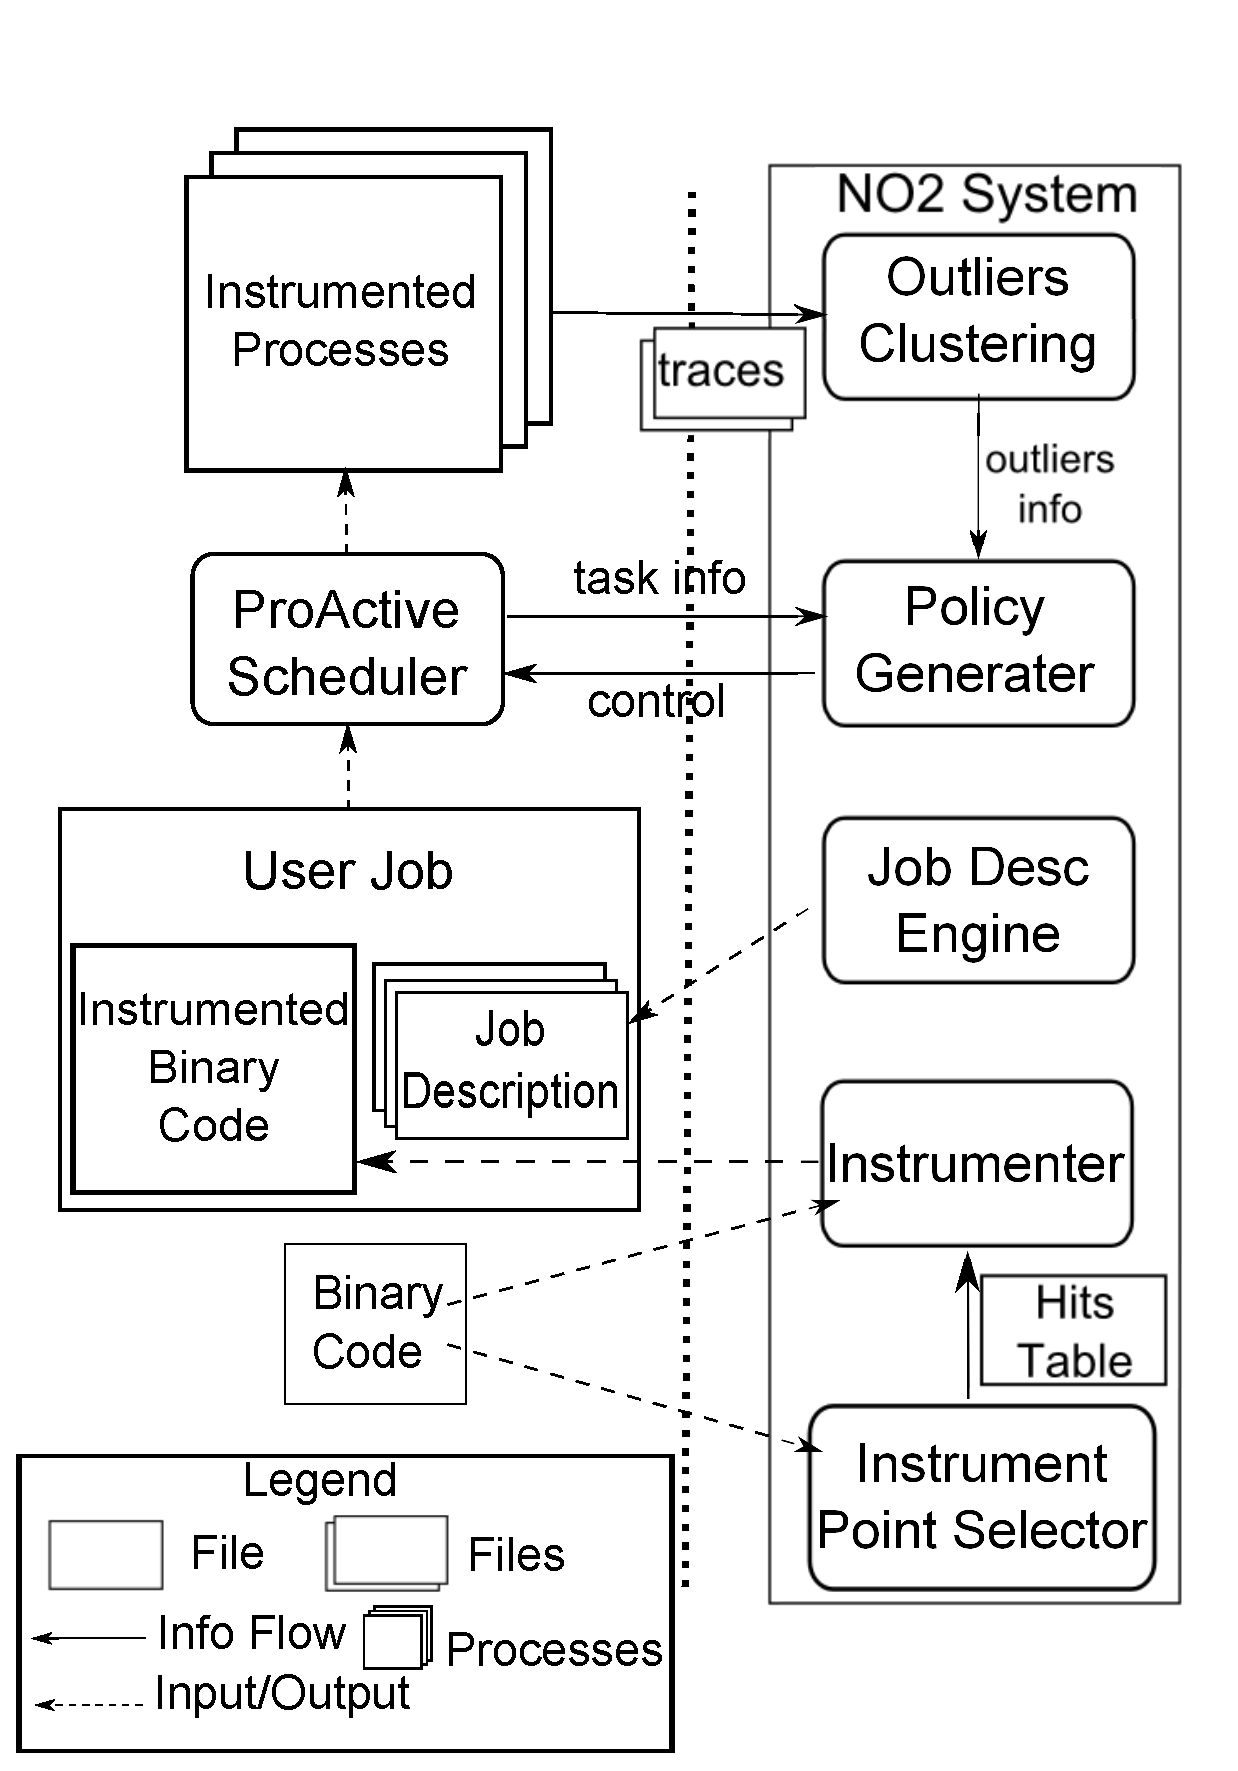
\includegraphics[width=0.9\columnwidth]{figures/NO2_arch.eps}
\caption{NO2 Architecture}
\label{figure:no2arch}
\end{figure}

We carefully designed NO2 to make sure of its independence with job scheduler which benefits users adapting to different job scheduler easily. As Figure \ref{figure:no2arch} shown, The only interactive between NO2 and ProActive scheduler is the interface for obtaining task status information of a job and request to kill and start a job or task. These abilities can be easily satisfied by any Schedulers' control interface, such as control script provided by ProActive Scheduler or command line tools provided by Condor. 

The job description template we provide can be used immediately in ProActive Scheduler, Because of following ProActive Scheduler’s job description XML structured rules. But it doesn't mean something dependence, It’s easily to change to another scheduler with tiny modification on format. And except for XML descriptor, there are three extra shell scripts for splitting, wrapping native task and merging the results if needed. The shell scripts will be submitted and executed as normal tasks on job scheduler. 

Taking a picture rendering job for example, there may be three phases for this job: 1. splitting the image into small pieces, 2. rendering them in parallel, 3. merging the rendered parts. These three phases exactly match NO2‘s three shell script template : split script, operation script and merge script. Users just need to add a image cutting command into the split script, which may be optional for other jobs and modify the default procedure copy input files to the destinations as needed. In the operation script, the native task must be  expressed as a command, a daemon process for trace log transferring is also launched defaultly. When all parts of result has been collected, a merge image command added in the merge script, optional for other jobs too. As described above,  users has a extreme flexibility to make their native tasks massive parallel. On the other hand it means NO2 do not provided any file transfer or data placement service and so on, which have been provided by job schedulers or a distributed file system of cluster itself.

In the next three sections, we will mainly illustrate the design and implementation of instrumentation, function hits statistics, outliers clustering and task scheduling policy generate in NO2 system.